\chapter{Grundlagen}

\section{Mathematische Grundlagen}

Diese Sektion beschreibt die wesentlichen mathematischen Konzepte, die in dieser Arbeit zur Verwendung kommen.

\subsection{Koordinatensysteme}

Ein wesentliches Konzept bei der Verarbeitung räumlicher Daten ist die Verwendung von Koordinatensystemen.
Sie werden genutzt um die Positionen von Daten und Objekten im Raum zu beschreiben.
Koordinatensysteme können für sich alleine stehen oder relativ zu anderen Koordinatensystemen.
Im Dreidimensionalen besitzt ein Koordinatensystem drei verschiedene Achsen (x, y und z-Achse), die jeweils im 90 Grad Winkel zueinander ausgerichtet sind.
Rotationen im Raum werden beschrieben als Rotationen um die jeweiligen Achsen.
Welche Achse in welche Richtung zeigt ist nicht eindeutig definiert.
Es gibt jedoch verschiedene Standards beziehungsweise Konventionen wie das links- oder rechtshändische Koordinatensystem.
In ROS wird konventionell ein rechtshändisches Koordinatensystem, abgebildet in Abbildung \ref{fig:ros_coordinate_sys} dargestellt. Dies wird im Folgenden ebenfalls als Standard verwendet.

\begin{figure}
		\centering
		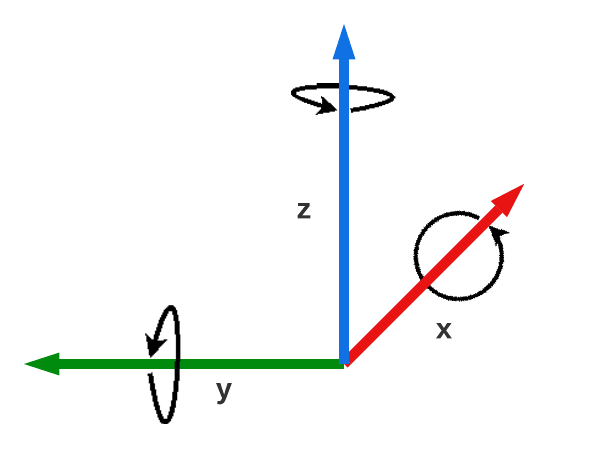
\includegraphics
			[scale=0.35]
			{ros_coordinate_sys}
		\caption
			[Caption for LOF]{Schematische Darstellung der Konvention für Koordinatensysteme im ROS Framework. Die z-Achse zeigt nach oben, die x-Achse nach vorne und die y-Achse nach links. Die Rotation um die Achsen ist entsprechend der Konvention im Uhrzeigersinn.}			                                                                                                                                     
		\label{fig:ros_coordinate_sys}
	\end{figure}

In der Robotik kommt es häufig vor, dass verschiedene (bewegliche) Komponenten relativ zu einem globalen Bezugssystem oder relativ zueinander beschrieben werden müssen. Die Bewegung eines übergeordneten Bezugssystems kann implizit für eine Veränderung der relativ zu diesem Bezugssystem platzierten Systeme führen.
Dies lässt sich anhand eines Arm-Roboters zeigen, der mehrere miteinander verbundene Gelenke hat. Bewegt sich ein Gelenk werden automatisch auch die am Arm weiter außen befindlichen Gelenke mitbewegt. Aus Sicht des bewegten, übergordneten Bezugssystems hat sich die Position der untergeordneten Gelenke nicht verändert, aus Sicht des globalen Bezugssystems, wie zum Beispiel dem Montierungspunkt des Roboters, allerdings schon.

In ROS werden Anhängigkeiten zwischen Bezugssystemen in einer Baumstruktur, genannt \textit{transformation tree (tf-tree)} dargestellt.
Die Wurzel dieser Baumstruktur ist das globale Bezugssystem, wie zum Beispiel der Ursprung einer globalen Karte oder der Startpunkt der Trajektorie eines Roboters.
Das globale Bezugssystem kann beliebig gewählt werden.
Auf diese Weise kann ein Koordinatensystem, welches relativ zu einem anderen gelegen ist im Baum als Kindknoten seinem Bezugssystem untergeordnet werden. Es wird nur die relative Transformation (s. Kapitel \ref{section:transformationen}) zwischen den Systemen im Baum gespeichert.
Dies hat den Vorteil, dass bei der Bewegung eines Systems die untergordneten Systeme nicht ebenfalls verändert werden müssen, da deren Transformationen relativ zum bewegten Bezugssystem angegeben sind und nicht global zur Wurzel des Baumes.
Abbildung \ref{fig:robot_tf} zeigt ein Beispiel für einen Roboter mit mehreren voneinander abhängigen System.


\begin{figure}
		\centering
		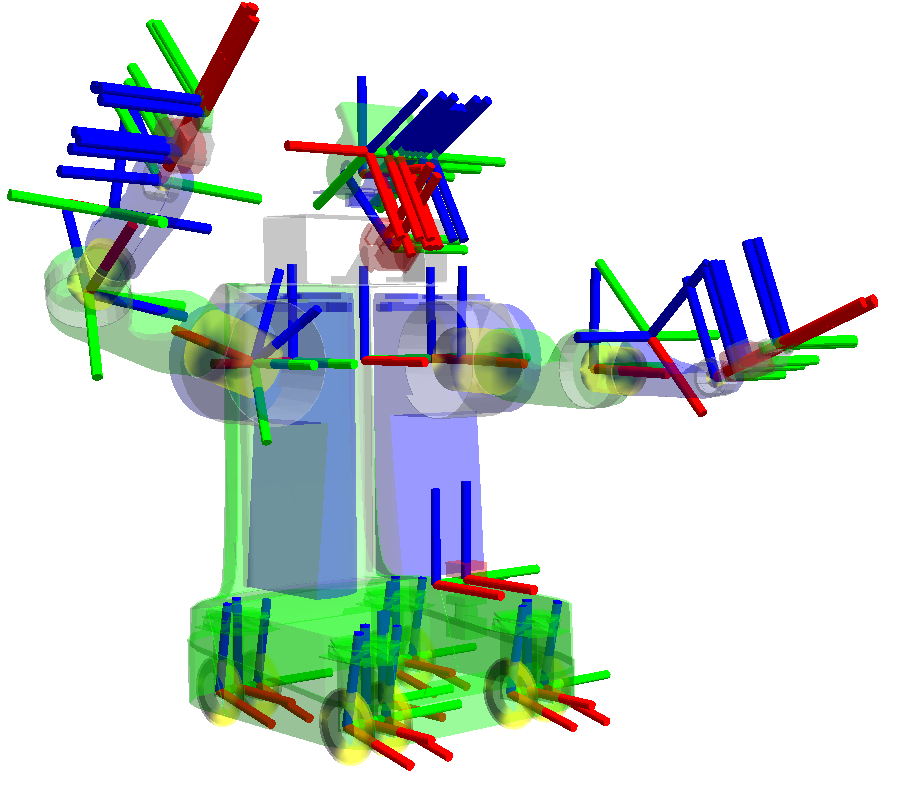
\includegraphics
			[scale=0.35]
			{robot_tf}
		\caption
			[Caption for LOF]{Schematische Darstellung eines Roboters und dessen beweglicher Teile. Die Ausrichtung der jeweiligen Gelenke wird mit einem lokalen Koordinatensystem beschrieben. Die globale Position einzelner Teile kann durch eine Verkettung der relativen Transformation in Richtung der Wurzel des Baumes bestimmt werden.
			Bild aus: TODO}			                                                                                                                                     
		\label{fig:robot_tf}
	\end{figure}

Auch räumliche Daten wie zum Beispiel Punktenwolken aus Laserscannern können relativ zu verschiedenen Koordinatensystemen gesehen werden.
So kann es nützlich sein die Punktwolke relativ zum Koordinatensystem des Scanners oder innerhalb des globalen Koordinatensystems zu betrachten. Um zwischen den Koordinatensystemen zu wechseln wird eine Koordinatensystemtransormation. Diese werden im folgenden Kapitel behandelt.

 
\subsubsection{Transformationen}
\label{section:transformationen}

Eine Koordinatensystemtransformation ist ein Sonderfall einer mathematischen Transformation, die eine Menge $X$ auf sich selbst abbildet:
\begin{myequation}
f: X \rightarrow X
\end{myequation}

Eine Koordinatensystemtransformation beschreibt die Differenz zwischen zwei unterschiedlichen Koordinatensystemen und enthält sowohl die Translationsdifferenz als auch die Rotationsdifferenz.
Zur Berechnung dieser Transformation zwischen zwei beliebigen Koordinatensystem $C_1$ und $C_2$ wird die absolute Translation und Rotation beider Koordinatensysteme zum Ursrungskoordinatensystem, wie zum Beispiel den Urpsrung einer Umgebungskarte, benötigt.
Durch diese Rotations und Translationskomponenten beschreibt sich die absolute Position und Rotation der Koordinatensysteme im Raum aus Sicht des Ursprungskoordinatensystems $C_{MAP}$. Diese absolute Position und Rotation ist die Transformation von den jeweiligen Koordinatensystemen ins Urpsrungskoordinatensystem.

Es existieren diverse Darstellungsweisen für Koodinatensystemtransformationen. Die intuitivste Weise der Darstellung ist die Darstellung als Vektor. In folgendem ist die Transformation vom Koordinatensystem $C_X$ ins Koordinatensystem $C_{MAP}$ dargestellt. Die Variablen $t_i$ bezeichnen dabei die Translationskomponenten und die Variablen $r_i$ die Rotationskomponenten um die jeweiligen Achsen. 

\begin{myequation}
T_{C_X \rightarrow C_{MAP}} = \colvec{t_x\\t_y\\t_z\\r_x\\r_y\\r_z}
\end{myequation}

Neben der Vektordarstellung kann eine Transformation zusätzlich als eine $4x4$ Matrix dargstellt werden.
Diese Darstellungsweise hat den Vorteil, dass die Transformation direkt per Matrixmultiplikation auf Daten wie um homogene Koordinaten erweiterte Punktdaten angewandt werden kann.
Auch die direkt Kombination verschiedener Transformationen ist durch eine Matrixmultiplikation möglich. Hier gilt es zu beachten, dass Matrixmultiplikation nicht kommutativ ist und ein Vertauschen der Reihenfolge bei der Multiplikation zu unterschiedlichen Ergebnissen führen kann.
Bei einer Verkettung von Transformationen durch Multiplikation wird die Matrix zuerst angewandt, welche am Ende der Multiplikation steht.

In dieser Arbeit werden Transformationen zum Beispiel verwendet um zu bestimmen, wie sich ein Roboter zwischen zwei Messungen bewegt hat. Diese Transformationen beschreiben relative Differenzen zwischen Roboterpositionen im Raum. Diese Roboterpositionen werden auch \textbf{Posen} genannt.
Eine Pose ist dabei eine meist absolute Beschreibung der Translation und Rotation eines Roboters zu einem gewissen Zeitpunkt $t$ aus Sicht des Ursprungskoordinatensystems wie zum Beispiel dem Map-Ursprung $C_{MAP}$.


\begin{figure}
		\centering
		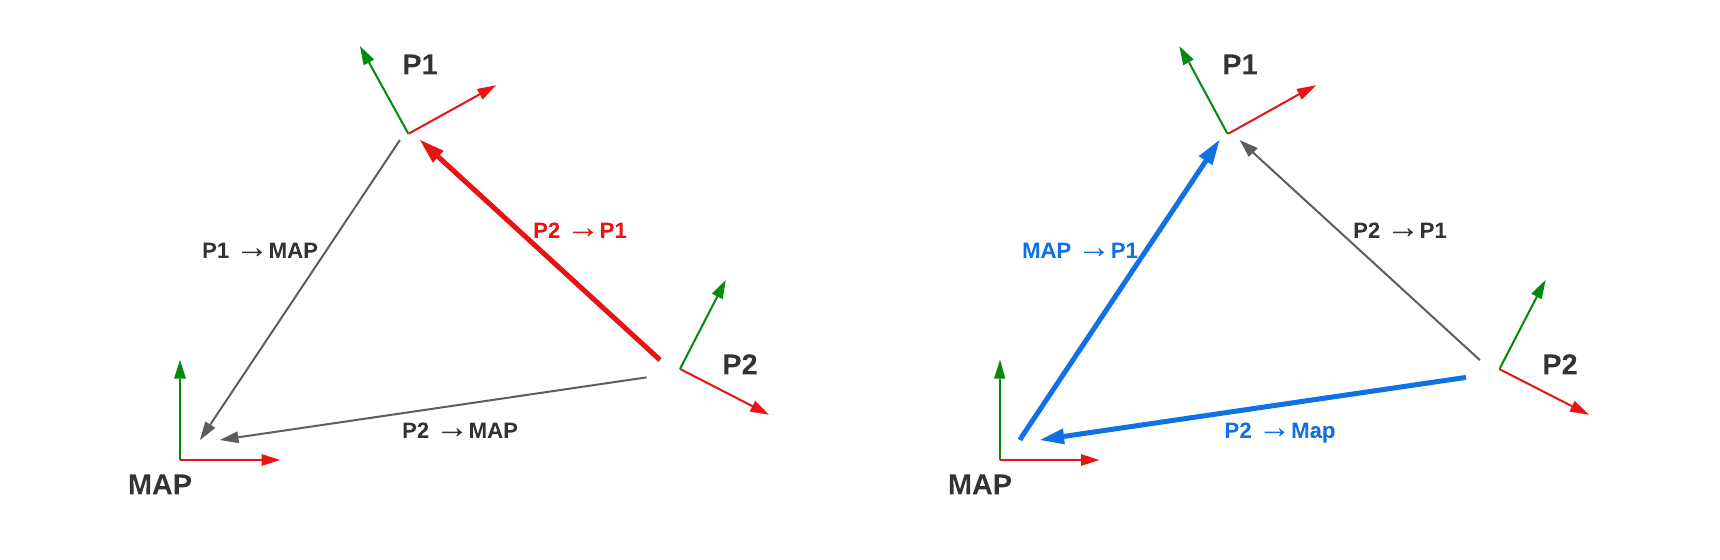
\includegraphics
			[scale=0.25]
			{transformation}
		\caption
			[Caption for LOF]{Schematische Darstellung der bestimmung einer Transformation zwischen zwei Roboter-Posen $P_1$ und $P_2$, hier zur Vereinfachung dargestellt in 2D. Gesucht ist die Transformation $\left( T_{P_2 \rightarrow P_1} \right)$. Diese kann implizit bestimmt werden durch eine Verkettung der Transformationen $T_{P_2 \rightarrow MAP}$ und $T_{MAP \rightarrow P1}$, hier dargestellt im rechten Teil der Abbildung in blau. Die Transformation $T_{MAP \rightarrow P1}$ ist dabei nicht explizit gegeben. Sie kann berechnet werden durch eine Inversion der Transformation $T_{P1 \rightarrow MAP}$. Die finale Gleichung zur Berechnung der relativen Transformation ist dargestellt in Gleichung \ref{equation:transformation}.}			                                                                                                                                     
		\label{fig:transformation}
	\end{figure}


Abbildung \ref{fig:transformation} zeigt die Mathematik hinter der Berechnung der Posedifferenz exemplarisch. Es wird deutlich, dass eine gesuchte Transformation aus dem Koordinatensystem von Pose $P_2$ in das Koordinatensystem von Pose $P_1$  $\left( T_{P_2 \rightarrow P_1} \right)$ gegeben ist durch:

\begin{myequation}
\label{equation:transformation}
\left( T_{P_2} \rightarrow T_{P_1} \right) = \left(T_{P_1 \rightarrow MAP} \right)^{-1} * T_{P_2 \rightarrow MAP}
\end{myequation}

\section{SLAM}

1. Grundlagen von SLAM beschreiben
-> Varianten des SLAM
-> Bezug zu HATSDF-SLAM
2. Vorraussetzungen (Repräsentationen für Posen (Pfad) und Umgebung)
3. Überleitungen in weitere Sektionen machen
	-> Loop Closure als mögliche Verbesserung des SLAM
	-> TSDF als Kartenrepräsentation
		-> auf Vorteile von TSDF eingehen (z.B. einfache Integration in Marching Cubes Algorithmus)


\section{Loop Closure}
\label{section:loop_closure_basics}

Warum wird Loop Closure benötigt?
Welchen Mehrwert gibt es?
Wie wäre ein grundlegendes vorgehen?
verweisen auf Loop-Closure Kapitel

\section{TSDF}